\section{Evaluation}
\FloatBarrier%

To recap the previous sections, we are dealing with two models here:
\begin{itemize}
  \item ``WordCNN'', a convolutional neural network operating on tokenized words
    and punctuation,
  \item ``CharCNN'', a convolutional neural network operating on tokenized
    characters,
\end{itemize}
as well as three variations for each model:
\begin{itemize}
  \item No clustering.
  \item The data is augmented with K-Means clustering.
  \item The data is augmented with clustering through an infinite mixture model.
\end{itemize}
These variations will be referred to as ``Baseline'', ``K-Means'' and ``Infinite
Mixture model'' respectively. Although K-fold cross validation would seem to be
a good way of comparing their relative performance, there are two properties of
cross validation that make it less desirable in this case:
\begin{itemize}
  \item The size of the training set is an interesting variable to test, but
    with cross validation it is directly tied to the number of iterations (e.g.\
    with a dataset of 1000 samples and 10 folds, each fold would have a
    training set of 100 samples).
  \item The training set and the test set are sampled from the same pool of
    data. In our case, we want the training set and the test set to be sampled
    from different electoral periods, because:
    \begin{itemize}
      \item A change of electoral period means at least a partial change in
        parliamentary members, which reduces the ability of the model to 
        overfit on the names of members.
      \item Although older documents use the same layout as newer ones, the PDF
        files were generated using different software (electoral period 13 started
        in 1994 and was the first period to use truly  digital documents --- older
        documents are scanned versions of printed paper). Since PDF
        decompilation is already a flaky process, this results in the 
        PDF decompiler making different mistakes than it does on the newer
        documents. This is a big problem for rule-based systems, but hopefully the
        probabilistic nature of neural networks makes them more robust to this issue.
    \end{itemize}
\end{itemize}
Therefore, a variation of cross validation is used instead. There is a pool of
training data consisting of documents from the 18th electoral period of the
\emph{Bundestag}, and a test set containing documents from the
electoral periods \numrange{13}{17}.
For 5 iterations, $k$ samples are pulled from the pool of training data. Each
of the three models is trained on these samples and then tested on the full test
set.

\subsection{Parameter Exploration\label{sec:param}}
Before directly comparing the two models, a good baseline value has to be
determined for the two parameters in the model that are the most difficult to
determine:
\begin{enumerate}
  \item the size of the sliding window applied to the lines of text in the input data
  \item the number of clusters to detect in the blocks of text (i.e.\ the ``k''
    in k-means)
\end{enumerate}
Although there are more parameters, they are related to the 
neural network, meaning there is a large amount of prior knowledge available to
set the parameters.

\todo[inline]{Plot opnieuw genereren met een logischere unit op de x-as, en
testen met window sizes die alleen naar voren kijken}
The effect of the sliding window size is shown in \cref{fig:window}. In this
figure, the window size refers to how many neighbouring lines of text are
considered: 0 means just the line of text by itself, 1 means the next line is
included, 2 means both the next and previous lines are included, et cetera.
For each model, there is a very sharp increase in performance when going from
zero to one neighbouring element, followed by a gradual decline as more elements
are added.
\begin{figure}[p]
  \centering
  \begin{subfigure}[b]{\textwidth}
    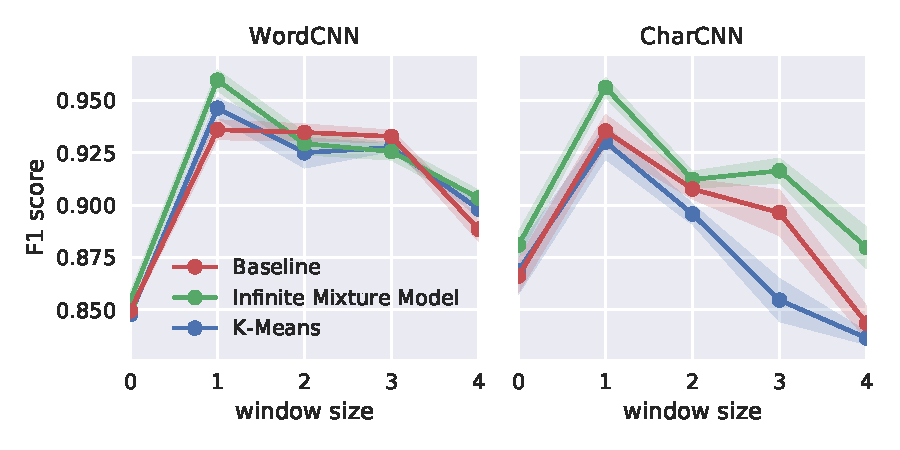
\includegraphics[width=\textwidth]{figures/results/2000-windowsize-old/tseries_f1.pdf}
    \caption{The F1 score with regards to the sliding window size for each
    model.\label{fig:window}}
    \vspace*{\fill}
  \end{subfigure}
  \begin{subfigure}[b]{\textwidth}
    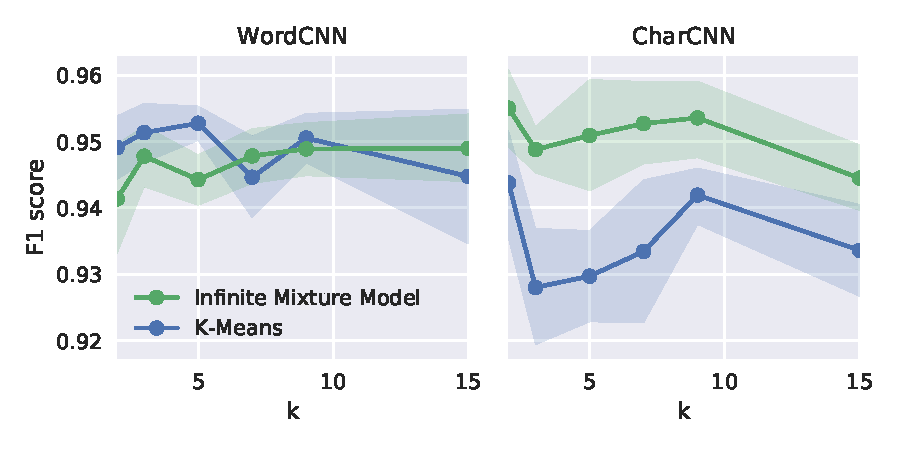
\includegraphics[width=\textwidth]{figures/results/2000-numclusters-old/tseries_f1.pdf}
    \caption{The F1 score with regards to the number of clusters for the K-Means
      model.\label{fig:numcluster}}
  \end{subfigure}
  \caption{These figures show the performance with regards to the sliding window
    size and the number of clusters, using a training set of 2000 samples. In
    \cref{fig:window}, the K-Means model was trained using 9 clusters.
    Each figure's F1 score is averaged over 5 trials; the translucent bands
    around the lines indicates the confidence intervals, meaning that based on
    the observed F1 scores and assuming normality, the true mean is 95\% likely
    to fall within that interval. The dots on the lines indicate
    measurements.\label{fig:params}
  }
\end{figure}

Results for the number of clusters are given in \cref{fig:numcluster}. In
this case, the window size was fixed to the previously determined optimum of 2.
The baseline model is not tested here due to not using clustering, and the
model using infinite mixture clustering is not tested due to its fixed amount of
clusters. The result varies little, and given the large variances no value can
really be said to outperform the rest.
\begin{figure}[tb]
  \centering
  \caption{This figure shows the performance with regards to the number of
    cluster types for each model trained on 1200 training samples with a window
    size of 5.  The vertical axis shows the F1 score, averaged over 10 trials;
    the horizontal axis shows the number of cluster types considered in the
    final clustering step.  The translucent bands around the lines indicates the
    confidence intervals, meaning that based on the observed F1 scores and
    assuming normality, the true mean is 95\% likely to fall within that interval.
    The dots on the lines indicate measurements.\label{fig:numcluster}}
\end{figure}

\subsection{Training Set Size}
Using the ideal parameters obtained in \cref{sec:param}, the influence of the
training set size is shown in \cref{fig:size}. This shows a number of
interesting differences. First of all, the Baseline and K-Means models perform
similarly for both CNN models at every input size, while the infinite mixture
version outperforms them only when using the CharCNN model. Additionally, the
WordCNN and CharCNN models respond much differently to variations of the
training set's size; WordCNN maxes out its performance at roughly 800 samples,
while CharCNN requires around 2000 samples to reach the same performance.
However, when augmented using the infinite mixture model, CharCNN peaks at a
slightly higher score than WordCNN.
\begin{figure}[tb]
  \centering
  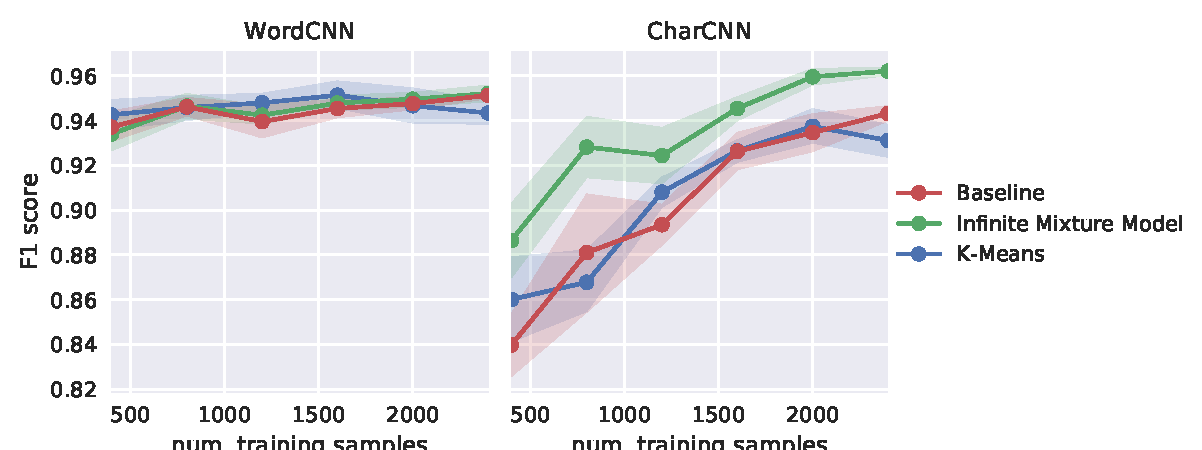
\includegraphics[width=\textwidth]{figures/results/training-size-old/tseries_f1.pdf}
  \caption{This figure shows the performance with regards to the size of the
    training set, using a window size of 2 of 9 clusters for the K-Means models.
    The F1 scores are averaged over 5 trials; the translucent bands
    around the lines indicates the confidence intervals, meaning that based on
    the observed F1 scores and assuming normality, the true mean is 95\% likely
    to fall within that interval. The dots on the lines indicate
    measurements.\label{fig:size}}
\end{figure}

\FloatBarrier%

%%% Local Variables:
%%% mode: latex
%%% TeX-master: "report"
%%% End:
